\chapter[Execução à nível de programa]{Execução à nível de programa}

Esse tópico representa as atividades e resultados obtidos pela equipe durante a execução do processo definido a nível de programa.

\begin{figure}[H]
    \centering
    \caption{Desenvolver programa}
    \label{processoPrograma}
    \includegraphics[keepaspectratio=true,scale=0.5]{figuras/processoPrograma.eps}
\end{figure}
\section{Reuniões realizadas}

Foram realizadas duas reuniões, entre a equipe e o PO, para obter as informações necessárias do nível de programa, todas foram não presenciais.

\subsection{Reunião 01-Programa}
    \indent \textbf{Data de execução:} 27/05/2016\\
    \indent \textbf{Objetivo da reunião:} elicitar características do sistema.\\
    \indent \textbf{Técnica de elicitação:} foi utilizada um conjunto de técnicas sendo estas:
    \begin{itemize}
        \item Brainstorming: é uma técnica utilizada para resolver problemas específicos, para reunir conhecimentos e gerar novas ideias ou projetos.
        \item Prototipagem: é uma implementação parcial de um sistema de forma rápida, sendo utilizado o protótipo de papel para identificar ou esclarecer a caractística levantada.
    \end{itemize}
    \indent \indent \textbf{Execução da técnica:} a reunião teve duas partes, sendo estas:\\
    \indent \textbf{Resumo da primeira parte:} nesta parte, a equipe junto ao cliente, utilizou, inicialmente, a técnica de brainstorming. Os assuntos descritos pelo diagrama de causa e efeito, representado pela imagem \ref{fishBone}, foram utilizados como temas para a execução da técnica e para direcionar a dinâmica foi utilizado um facilitador, membro da equipe de requisitos.\\
    \indent \textbf{Resumo da segunda parte:} nesta parte, foi utilizada a técnica de prototipagem, para auxiliar o entendimento de certas características levantadas na primeira parte da reunião. Utilizando a ferramenta paint, foi feito alguns protótipos de telas pelos integrantes da equipe de requisitos em conjunto com o cliente.\\
    \indent A prototipagem ajudou a complementar a ideia das features. Os protótipos gerados nessa reunião estão apresentados pelas images:  \ref{prototipo01}, \ref{prototipo02}, \ref{prototipo03}, \ref{prototipo04}.\\
    \indent \textbf{Resultado da reunião:} ao término da reunião, foi possível definir as features do Business EP01, Business EP02 e Enable EP03. Gerando assim o backlog de features dos 3 épicos.\\

\begin{figure}[H]
    \centering
    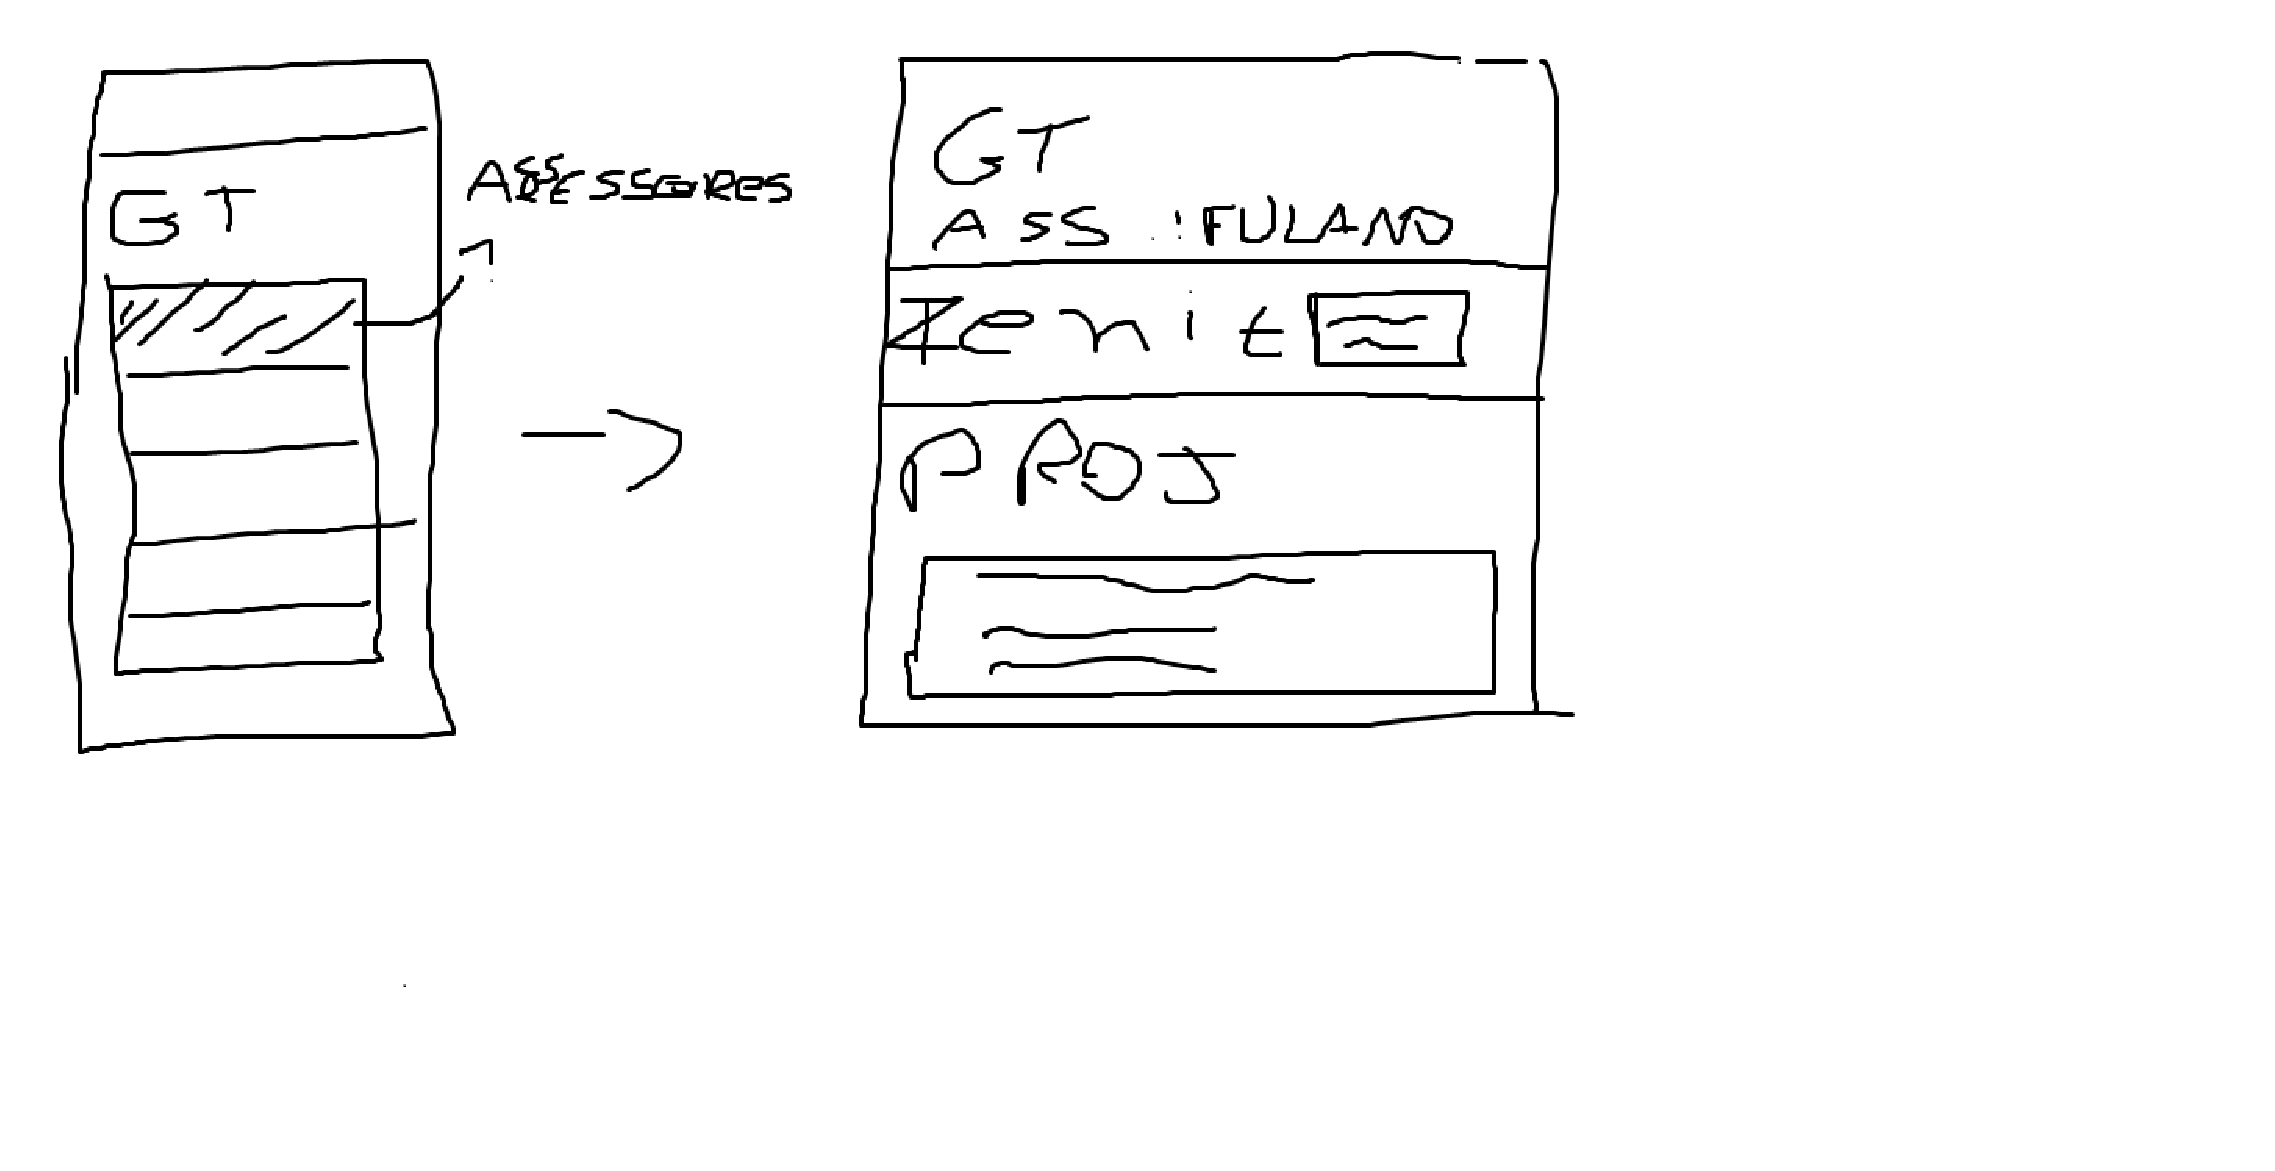
\includegraphics[keepaspectratio=true,scale=0.3]{figuras/prototipo01.eps}
    \caption[Prototipo 1 de feature]{Protótipo 1 para elicitação de feature\label{prototipo01}}
\end{figure}
\begin{figure}[H]
    \centering
    \includegraphics[keepaspectratio=true,scale=0.3]{figuras/prototipo02.eps}
    \caption[Prototipo 2 de feature]{Protótipo 2 para elicitação de feature\label{prototipo02}}
\end{figure}
\begin{figure}[H]
    \centering
    \includegraphics[keepaspectratio=true,scale=0.3]{figuras/prototipo03.eps}
    \caption[Prototipo 3 de feature]{Protótipo 3 para elicitação de feature\label{prototipo03}}
\end{figure}

\begin{figure}[H]
    \centering
    \includegraphics[keepaspectratio=true,scale=0.3]{figuras/prototipo04.eps}
    \caption[Prototipo 4 de feature]{Protótipo 4 para elicitação de feature\label{prototipo04}}
\end{figure}

\subsection{Reunião 02-Programa}

    \indent \textbf{Data de execução:} 01/06/2016\\
    \indent \textbf{Objetivo da reunião:} verificar e validar com PO as \textit{features} elicitadas e confirmar se estes estão de acordo com os interesses do cliente e negociar possíveis modificações. Realizar a priorização das features de acordo com seus interesses.\\
    \indent \textbf{Resultado da reunião:} o PO concordou com todas a \textit{features} e priorizou o \textit{backlog} do programa de acordo com seus interesses.\\

Após a priorização feita pelo cliente, a equipe técnica avaliou e percebeu que havia relação de dependência horizontal entre os requisitos. No qual a feature “gerenciar informações acadêmicas” que era a maior prioridade do PO, teria que vir depois da “gerenciar informações pessoais”. Dessa forma, foi negociado a troca na ordem de implementação destas duas e ele concordou.\\

Logo, confirmou-se e priorizou-se as \textit{features} e assim foi obtivemos o resultado do backlog priorizado do a nível de programa.\\

\section{Backlog de Programa}

O backlog a seguir foi elaborado a partir das reuniões com o \textit{Product Owner} até o presente momento da execução do processo. O backlog do apêndice \ref{backlogFeatures} possui as features ao final da execução do processo, ou seja, contém mudanças que foram realizadas após esta etapa do relatório.

\subsection{Business EP01}
\textbf{Business}
\begin{itemize}
    \item FT01 Gerenciar informações pessoais
    \item FT02 Gerenciar informações acadêmicas
    \item FT03 Gerenciar informações profissionais
    \item FT04 Gerenciar informações de projetos
\end{itemize}
\textbf{Enable}
\begin{itemize}
    \item FT05 Integração com módulo de projetos
    \item FT06 Controle de perfil de acesso
\end{itemize}
\subsection{Business EP02}
\textbf{Business}
\begin{itemize}
    \item FT07 Gerenciamento da evolução de perfis profissionais
    \item FT08 Acompanhamento motivacional dos membros
    \item FT09 Suporte ao acompanhamento dos gestores
    \item FT10 Acompanhamento de presença
\end{itemize}
\subsection{Enable EP03}
\textbf{Enable}
\begin{itemize}
    \item FT11 Padrão arquitetural da aplicação web Model-View-Controller
    \item FT12 Disponibilidade do serviço
    \item FT13 Interfaces de interação responsivas
\end{itemize}
\section{Visão}

Tradicionalmente, os requisitos de um produto de software são representados em forma de um documento dando uma visão geral do sistema. Em metodologias ágeis, mesmo não tendo foco em documentação, um documento que representa a visão geral do produto é bem aproveitado com essa finalidade \cite{leffingwell2011}. O documento de visão do sistema é abordado no apêndice \ref{docVisao}.

\section{Roadmap}

O roadmap foi planejado para entregar um conjunto de \textit{features} em ordem de priorização.

\textbf{Release 12/06/2016 a 10/07/2016}
\begin{itemize}
    \item Enable FT06 Controle de perfil de acesso
    \item Enable FT11 Padrão arquitetural da aplicação web Model-View-Controller
    \item Business FT01 Gerenciar informações pessoais
    \item Business FT02 Gerenciar informações acadêmicas
    \item Enable FT13 Interfaces de interação responsivas
\end{itemize}
\textbf{Release 10/07/2016 a 07/08/2016}
\begin{itemize}
    \item Enable FT12 Disponibilidade do serviço
    \item Business FT03 Gerenciar informações profissionais
    \item Business FT04 Gerenciar informações de projetos
    \item Enable FT05 Integração com módulo de projetos
\end{itemize}
\textbf{Release 07/08/2016 a 04/09/2016}
\begin{itemize}
    \item Business FT07 Gerenciamento da evolução de perfis profissionais
    \item Business FT08 Acompanhamento motivacional dos membros
    \item Business FT09 Suporte ao acompanhamento dos gestores
    \item Business FT10 Acompanhamento de presença
\end{itemize}
